\section{Implementation of the Safety Annex}
\label{sec:impl}
%Important features were considered before the implementation of the safety annex; these we addressed one by one and will outline below. 

As described in Section~\ref{sec:concepts}, an AADL~\cite{AADL_Standard} model describes a system in terms of a hierarchy of components and their interconnections, where each component can either represent a logical entity (e.g., application software functions, data) or a physical entity (e.g., buses, processors). AADL is used to specify and analyze real-time embedded systems. It includes specifications specific to hardware, software, and system component abstractions. The language definition is sufficiently rigorous to support formal analysis tools that allow for early phase error/fault detection~\cite{FeilerModelBasedEngineering2012}. 

\begin{figure}[h!]
	%\vspace{-0.1in}
	\begin{center}
	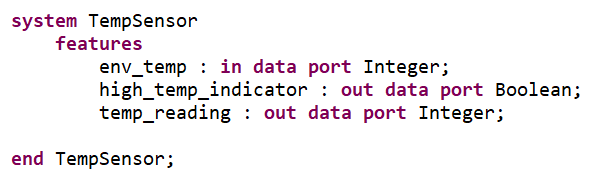
\includegraphics[width=.8\textwidth]{images/aadlComponent.png}
	\caption{AADL Component Types}
	\label{fig:aadlComponent}
	%\vspace{-0.2in}
	%\vspace{-0.1in}
	\end{center}
\end{figure}

Central to an AADL model are component \emph{types} and \emph{implementation} declarations. Figure~\ref{fig:aadlComponent} shows an example of a simple sensor component type defined in AADL. The component has an environmental temperature as input and two outputs: a high temperature indication and a temperature reading. In the type declaration, you define the category (\texttt{system} in this example) and features such as inputs and outputs; the implementation contains definitions of the internal structure of the component, e.g., internal constituents and their interactions. 

\begin{figure}[h!]
	%\vspace{-0.1in}
	\begin{center}
	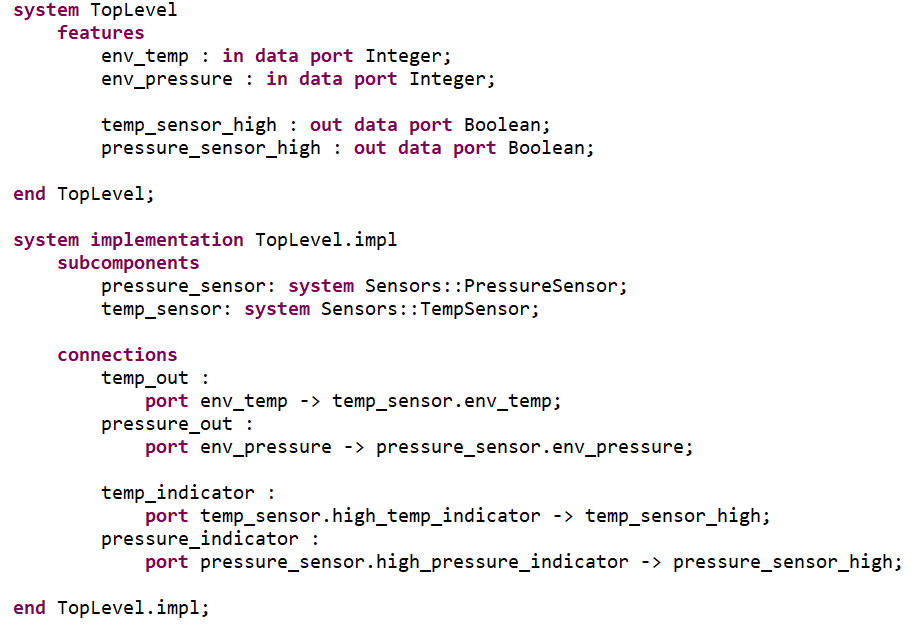
\includegraphics[width=1.0\textwidth]{images/aadlImplementation.png}
	\caption{An AADL Component Implementation Definition}
	\label{fig:aadlImplementation}
	%\vspace{-0.2in}
	%\vspace{-0.1in}
	\end{center}
\end{figure}

An implementation of the sensor component type is shown in Figure~\ref{fig:aadlImplementation}. The system contains a type of its own (top of figure: \texttt{system TopLevel}) which holds any environmental inputs or subcomponent outputs. The implementation defines the subcomponents of the system and their connections (bottom half of figure). 

Since AADL supports model-based system development and the language definition is sufficiently rigorous to support formal analysis tools that allow for early phase error/fault detection~\cite{FeilerModelBasedEngineering2012}, this language was chosen for this research. 

As described in Section~\ref{subsec:mbsa}, {\em nominal model analysis} is a part of the MBSA process. The nominal model consists of the system model architectural design as well as behavioral contracts for each component and requirement specifications. The verification at the nominal level consists of showing that the model satisfies the specified requirements in the absence of faults. 

The Assume-Guarantee Reasoning Environment (AGREE)~\cite{cofer2012compositional} is a language annex for AADL that provides a mechanism for the specification of component requirements in formal logic and utilizes a model checker to provide proofs regarding these specifications as described in Section~\ref{sec:concepts}. 

\begin{figure}[h!]
	%\vspace{-0.1in}
	\begin{center}
	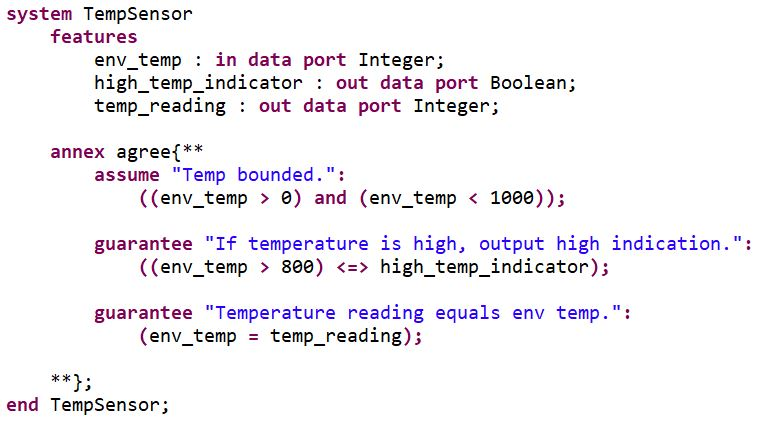
\includegraphics[width=1.0\textwidth]{images/agreeContract2.JPG}
	\caption{The AGREE Contract for an AADL Component Type}
	\label{fig:agreeContract}
	%\vspace{-0.2in}
	%\vspace{-0.1in}
	\end{center}
\end{figure}

An example of an AGREE contract is shown in Figure~\ref{fig:agreeContract} and is placed in the context of the AADL temperature sensor component shown in Figure~\ref{fig:aadlComponent}.  An AGREE contract consists of {\em assumptions} on the inputs of AADL components that constrain what the component sees from the environment and {\em guarantees} on the outputs that constrain how the component behaves given its environment. In this example, the assumption restricts the environmental temperature to be within a range of values; the guarantee defines the behavior of the component given the environment. 

Since our desire was to facilitate {\em behavioral error propagation}, AGREE was a suitable and obvious choice for the nominal verification tooling. 

Through AGREE, the nominal model is translated into the dataflow programming language Lustre~\cite{Halbwachs91:IEEE} that is used as input to the JKind model checker~\cite{2017arXiv171201222G}. JKind uses a series of backend SMT-solvers to generate proofs of the top level AGREE properties specified in the model. When there exists a trace such that a property is invalid, JKind provides a {\em counterexample} showing the system trace in which the property is violated. An example of this is shown in Figure~\ref{fig:coex}. 

\begin{figure}[h!]
	%\vspace{-0.1in}
	\begin{center}
	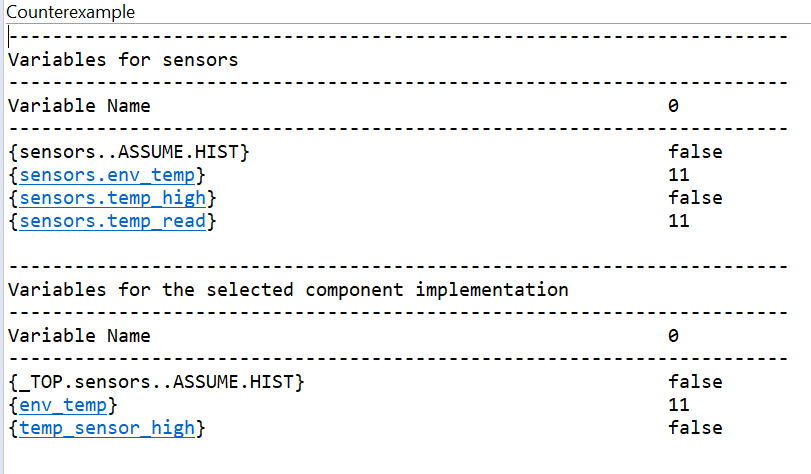
\includegraphics[width=1.0\textwidth]{images/coex.png}
	\caption{A Counterexample to an Invalid Property}
	\label{fig:coex}
	%\vspace{-0.2in}
	%\vspace{-0.1in}
	\end{center}
\end{figure}

The model checker takes an adversarial role in the proof process by trying to find paths such that the proof is violated. If none exist, then the results are valid. This adversarial role is exactly what we wished to harness for this kind of analysis. If we allow faults to be active, but leave them unconstrained, this allows the model checker to determine if certain faults could lead to a violation of a property. These counterexamples could then contain fault information. 

Given that AGREE guarantees define the {\em output} behavior of components, any connected component's assumptions rely on those guarantees. If an assumption is violated, the guarantee may not hold. By associating a fault with the output of a component, this fault -- when active -- may violate assumptions and guarantees along the signal flow within a system. This was our goal; we wished to view the behavioral propagation of an active fault. 

\subsection{Implementation Architecture}
\label{sec:implArchitecture}
The safety annex is written in Java as a plug-in for the OSATE AADL toolset, which is built on Eclipse.  It is not designed as a stand-alone extension of the language, but works with behavioral contracts specified using the AGREE annex for AADL~\cite{NFM2012:CoGaMiWhLaLu}. 
The architecture of the Safety Annex is shown in Figure~\ref{fig:plugin-arch}.

\begin{figure}[h]
	\begin{center}
		%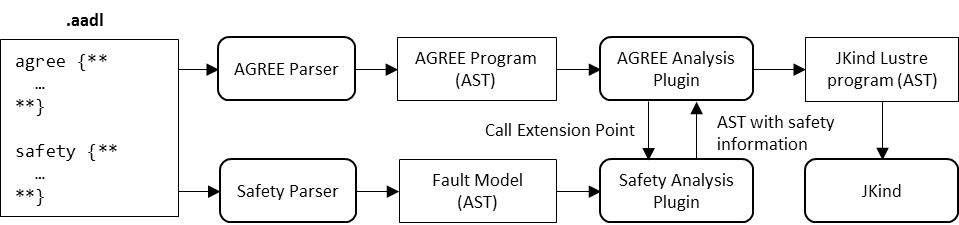
\includegraphics[trim=0 400 430 0,clip,width=0.85\textwidth]{images/arch.png}
		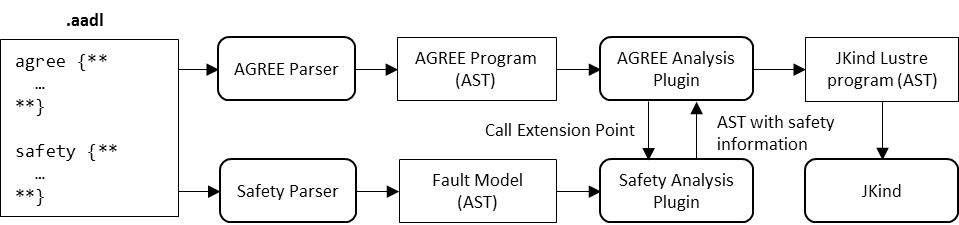
\includegraphics[width=\textwidth]{images/arch.png}
	\end{center}
	%\vspace{-0.2in}
	\caption{Safety Annex Plug-in Architecture}
	\label{fig:plugin-arch}
	%\vspace{-0.2in}
\end{figure}

The safety language extension resides in an annex of AADL and the faults defined therein are translated into an abstract syntax tree and inserted into the AGREE program. The AGREE program contains the building blocks for the translation into Lustre which is the program directly analyzed by JKind.  

When performing fault analysis, the fault definitions defined in the safety annex extend the AGREE contracts to allow faults to modify the behavior of component outputs. The temperature sensor subcomponent shown in Figure~\ref{fig:agreeContract} encoded into Lustre is shown in Figure~\ref{fig:lustreTempNode}\footnote{The Lustre code is slightly simplified for readability.}.

\begin{figure}[h]
	\begin{center}
		%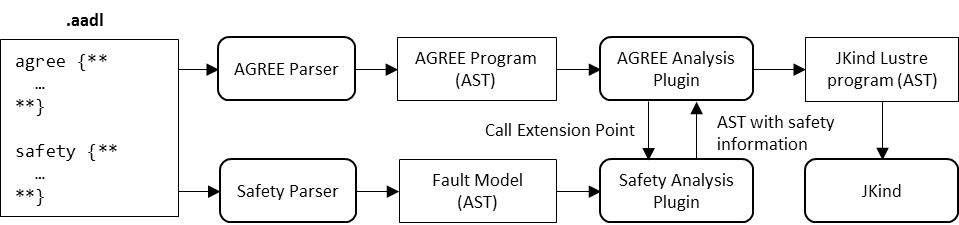
\includegraphics[trim=0 400 430 0,clip,width=0.85\textwidth]{images/arch.png}
		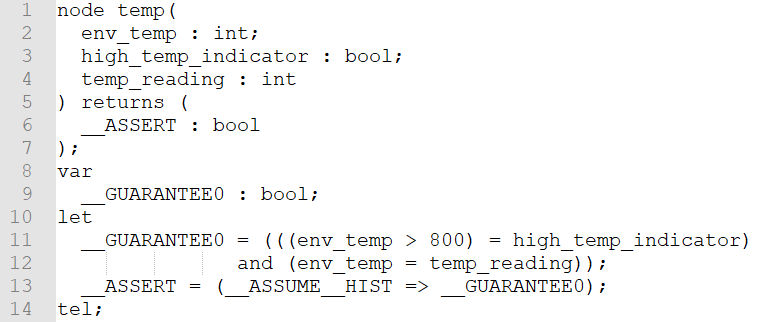
\includegraphics[width=0.8\textwidth]{images/lustreTempNode.png}
	\end{center}
	%\vspace{-0.2in}
	\caption{Temperature Component in Lustre}
	\label{fig:lustreTempNode}
	%\vspace{-0.2in}
\end{figure}

The inputs and outputs (lines 2-4) correspond directly to the AADL inputs and outputs of the component; likewise, the guarantee (\texttt{\_\_GUARANTEE0}) corresponds to the guarantee on the outputs. The \texttt{\_\_ASSERT} statement on line 13 states that as long as the assumptions hold, the guarantee is implied. 

From the perspective of fault analysis, we want to insert a fault on the output of the component. This fault may or may not be active -- it is up to the model checker. To this end, we specify three variables per potentially faulty output: \texttt{fault\_nominal}, \texttt{fault\_trigger}, and \texttt{fail\_val}. If the trigger is true, then output failure value, else output nominal value. This can be seen in Figure~\ref{fig:lustreTempNodeFault}: the new variables are assigned as inputs (lines 4-6) and the assert statement in line 20 shows the triggering behavior.

\begin{figure}[h]
	\begin{center}
		%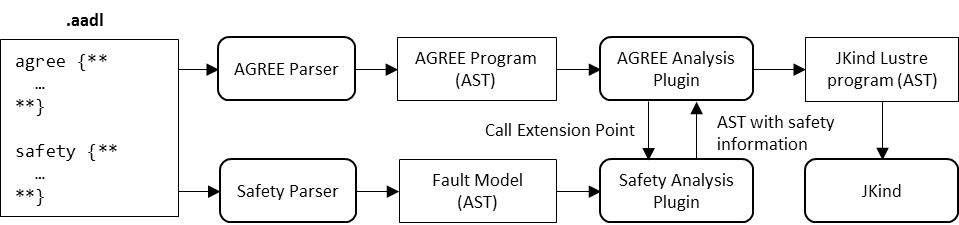
\includegraphics[trim=0 400 430 0,clip,width=0.85\textwidth]{images/arch.png}
		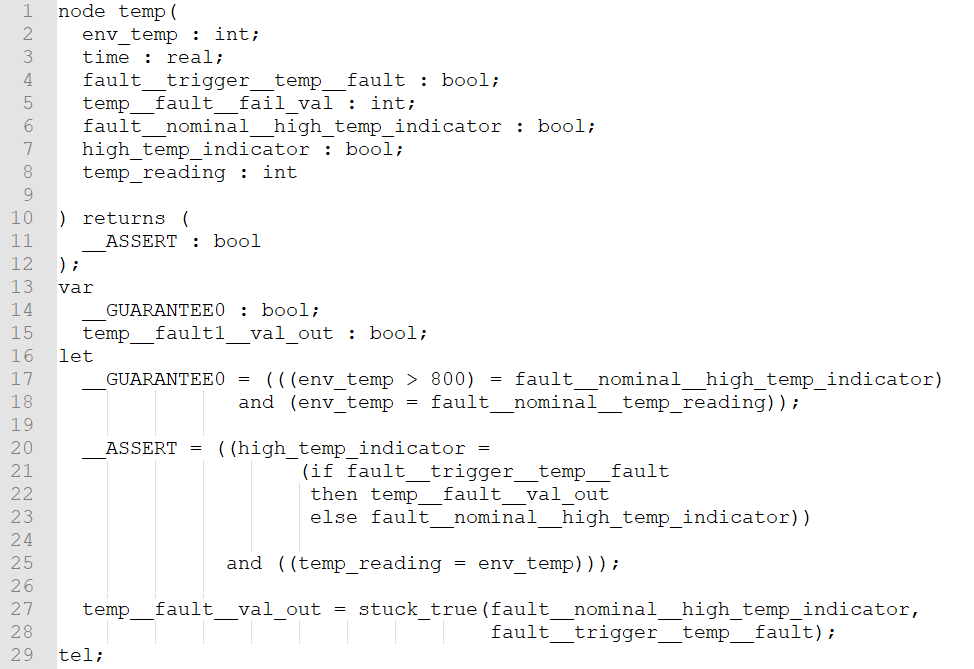
\includegraphics[width=0.8\textwidth]{images/lustreTempNodeFault.png}
	\end{center}
	%\vspace{-0.2in}
	\caption{Temperature Component with Fault in Lustre}
	\label{fig:lustreTempNodeFault}
	%\vspace{-0.2in}
\end{figure}

This allows for the possibility of active faults, but when the faults are inactive, the nominal value is simply passed through. Line 27 of Figure~\ref{fig:lustreTempNodeFault} shows a call to what we call a {\em fault node}; this is the code that specifies the behavior of an active fault. The fault node \texttt{stuck\_true} is shown in Figure~\ref{fig:lustreFaultNode}. The behavior of an active fault is to output {\em true}. The \texttt{trigger} input to the fault node corresponds directly with the trigger defined in the temperature node of Figure~\ref{fig:lustreTempNodeFault} on line 4. 

\begin{figure}[h]
	\begin{center}
		%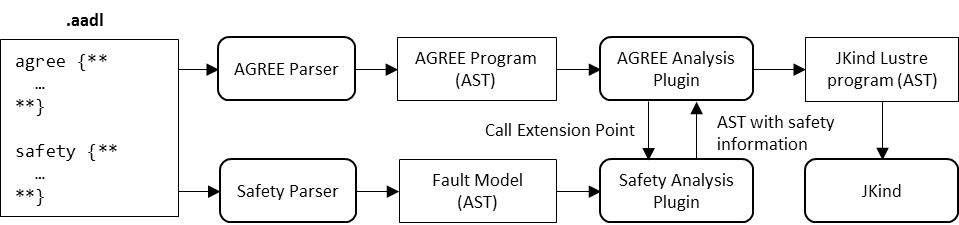
\includegraphics[trim=0 400 430 0,clip,width=0.85\textwidth]{images/arch.png}
		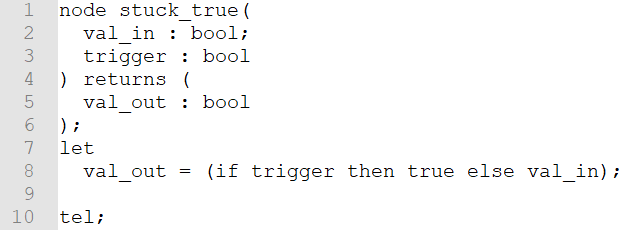
\includegraphics[width=0.8\textwidth]{images/lustreFaultNode.png}
	\end{center}
	%\vspace{-0.2in}
	\caption{A Fault Node in Lustre}
	\label{fig:lustreFaultNode}
	%\vspace{-0.2in}
\end{figure}
 
The model elements are translated into Lustre formulae. These are represented in JKind as a transition system, and reasoning is performed using $k$-induction. At each time-step of analysis, every formula in the model is given an assignment based on the constraints over that formula. If every assignment results in a provable property over $k$ steps of induction, the property holds. When performing safety analysis over the model, each fault is defined as an {\em activation literal} and is unconstrained. If the assignment to an activation literal is {\em true}, this corresponds to an active fault and potentially violated guarantee. If that assignment violates a guarantee, then this violation will be reflected in the analysis results. At a system level, it can be seen if a violated guarantee will in turn violate the top level property. Hence it is seen how active faults at leaf level components violate the system level properties. 

This analysis approach allows for implicit propagation of violations throughout the system. It also allows for arbitrary temporal activations of faults. There are no explicit constraints put on faults stating when an activation can occur, which allows the model checking procedure free reign to activate the faults at the worst possible times. If there are dependencies regarding fault activations, these are handled through the use of explicit error propagations (see Section~\ref{sec:propogation}).

The main constraint put on the model checker in terms of the activation of faults consist of {\em fault hypothesis statements}. These constrain the model by stating either the number of faults that may be active at once, or the overall probability threshold that is allowed. In the latter case, each fault has an associated probability; assuming independence, the probability of a set of faults occurring should not be less than the threshold defined. 

There are two different types of fault analysis that can be performed on a fault model: verification in the presence of faults or the generation of minimal cut sets. The Safety Annex plugin intercepts the AGREE program and adds fault model information depending on which type of fault analysis is being run. For more information on types of fault analysis, see Section~\ref{sec:analysisResults}.









